\documentclass[11pt]{article}

\usepackage{amsmath,amssymb,amsfonts}
\usepackage{graphicx}
\usepackage{pgfplots}
\usepackage{multicol}
\usepackage{enumitem}


\setlength{\topmargin}{-.5in} \setlength{\textheight}{9.25in}
\setlength{\oddsidemargin}{0in} \setlength{\textwidth}{6.8in}


\begin{document}

\Large


\noindent{\bf Name: \hfill Date: \hfill Exam 1 \hfill AP Calculus - Hargus}

\medskip\hrule
\vspace{10pt}

\noindent \textbf{Instructions:} Please \textbf{show all work} on the test paper (partial credit may be awarded for correct work, even if your answer is wrong). You may use the back side if you run out of room. Calculators are not allowed, but \textbf{simplify} your answers as much as you can. Cheating of any kind will result in a score of zero.


\begin{enumerate}[itemsep=30pt]

\item (6 points) What is the limit definition of the derivative of $f(x)$? (Note: we learned two ways of writing it in class, you can use either below)

$$f'(x) = \rule{5cm}{0.15mm}$$

\item (12 points) Evaluate the limit, if it exists (show any work involved):
\begin{multicols}{2}
\begin{enumerate}[itemsep=50pt]
    \item $\displaystyle{\lim_{x \to -5} -1}$ \\
    \item $\displaystyle{\lim_{x \to -3} x}$ \\
    \item $\displaystyle{\lim_{x \to 3} \frac{x - 3}{x^2 - 2x - 3}}$ \\
    \item $\displaystyle{\lim_{x \to -\infty} \sin{x}}$ \\
    \item $\displaystyle{\lim_{t \to 0} \frac{3^{2t} - 1}{3^t - 1}}$ \\
    \item $\displaystyle{\lim_{x \to \infty} \frac{x^3 +x}{x^2 + 1}}$ \\
\end{enumerate}
\end{multicols}

\vspace{50pt}

\item (6 points) Consider the function $f(x) = -|x| + 3$. True or false?
\begin{enumerate}
    \item \rule{1cm}{0.4pt} $f(x)$ has a horizontal asymptote at $y=3$.
    \item \rule{1cm}{0.4pt} $f(x)$ is continuous at $x=3$.
    \item \rule{1cm}{0.4pt} $f(x)$ is differentiable at $x=3$.
\end{enumerate}

\newpage

\item (30 points) Find the derivative $f'(x)$ (show any work and simplify where possible):
\begin{enumerate}[itemsep=25pt]
    \item{$f(x) = 6$} \\
    \item{$f(x) = x^3 + x + 6$} \\
    \item{$f(x) = 5\sqrt{x}$} \\
    \item{$f(x) = 2^x \sin(x)$} \\
    \item{$f(x) = (-x + 5)^4$} \\
    \item{$f(x) = \displaystyle{\frac{x^2}{e^x}}$} \\
    \item{$f(x) = e^{x^2}$} \\
    \item{$f(x) = \sin^2(x) + \cos^2(x)$} \\
    \item{$f(x) = \sin^{-1}(2x)$} \\
    \item{$f(x) = \ln(\cos(x))$} \\
\end{enumerate}

\newpage

\noindent{\bf Name: \hfill Date: \hfill Midterm 1 \hfill Calculus - Hargus}

\medskip\hrule


\item (12 points) Find the \textbf{second derivative} $y''$ for the given $y$ (show any work and simplify where possible):

\begin{enumerate}[itemsep=30pt]
    \item{$y = 10x^2 + 5x^3$} \\
    \item{$y = x \sin(x)$} \\
    \item{$y = x^{\frac{1}{3}}$} \\
\end{enumerate}

\item (6 points) If for $f(x)$ we know $\lim_{x \to 5} f(x) = \infty$, what kind of asymptote do we have (circle: \textbf{horizontal} or \textbf{vertical}) and what is the equation for that asymptote's line?

\begin{flushright}\noindent\rule{4cm}{0.4pt}\end{flushright}

\item (8 points) True or false?
\begin{enumerate}[itemsep=30pt]
    \item \rule{1cm}{0.4pt} $\sin^{-1}(x) = \frac{1}{\sin{x}}$
    \item \rule{1cm}{0.4pt} $\sin^{2}(x) = (\sin{x})^2$
    \item \rule{1cm}{0.4pt} If $y=f(x)$, then $f''(x) = y'' = \frac{d^2y}{dx^2}$
    \item \rule{1cm}{0.4pt} $\frac{d}{dx} \left( \tan^{-1} x \right) = \frac{1}{x^2 + 1}$
\end{enumerate}

\newpage

\item (10 points) Find $\frac{dy}{dx}$ (the derivative of $y$ with respect to $x$) for the following:
\begin{enumerate}[itemsep=70pt]
    \item $x^4 + y^4 = 1$
    \item $x^{\frac{1}{2}} + y^{\frac{1}{3}} = 3y$
\end{enumerate}

\vspace{30pt}

\item (10 points) For each graph below, draw the derivative function $f'(x)$ on the same graph below (does not need to be exact, though x-intercepts and sign ($+$/$-$) should be correct):

\vspace{10pt}
\hspace{50pt}(a)
\begin{center}
\begin{tikzpicture}
\begin{axis}[ xlabel={$x$}, ylabel={$y$}
  ,axis lines=middle
  ,samples=1000, grid, thick
  ,domain=-10:10
  ,axis equal
  ,legend pos=outer north east
  ,xmin=-5, xmax=5,
  ,ymin=-5, ymax=5
  ]
\addplot+[no marks] {(x+3)^2*(x-3)/20};
\addlegendentry{$f(x)$}
\end{axis}
\end{tikzpicture}
\end{center}

\vspace{10pt}
\hspace{50pt}(b)
\begin{center}
\begin{tikzpicture}
\begin{axis}[ xlabel={$x$}, ylabel={$y$}
  ,axis lines=middle
  ,samples=1000, grid, thick
  ,domain=-10:10
  ,axis equal
  ,legend pos=outer north east
  ,xmin=-5, xmax=5,
  ,ymin=-5, ymax=5
  ]
\addplot+[no marks] {sin(x*180/3.14) + 2};
\addlegendentry{$f(x)$}
\end{axis}
\end{tikzpicture}
\end{center}

\end{enumerate}

\end{document} 